\chapter{Modellierung}

Modellierung ist bei den meisten Informatikern kein sehr beliebtes Thema. Modellieren bedeutet sich zunächst hinzusetzen und das Programm was man schreiben möchte zu planen. Ich habe in den vergangenen Kapiteln bereits eine Notation dazu eingeführt in Grenzen eingeführt: Struktogramme.

Bislang habt ihr nur Programme geschrieben die sehr leicht zu überblicken und sehr schnell zu schreiben waren. Sobald ihr anfangt größere Programme zu schreiben ist das einfach drauflos schreiben schwieriger und führt zu meist zu schlechteren Ergebnissen wenn ihr vorher nicht euer Programm modelliert. Stell dir vor du sollst eine aus Informatikersicht verhältnismäßig einfache Anwendung wie Minesweeper implementieren. Dann brauchst du eine Oberfläche mit Bedienelementen, du brauchst einen Algorithmus der bei einem Klick ausrechnet welche Felder aufzudecken sind, du brauchst um den Nutzer zufrieden zu machen auch Highscores oder ähnliche Zusätze. Um das Programm effizient und möglicherweise im Team zu schreiben ist eine vorherige Planung oder Modellierung unerlässlich.

Ich möchte hier eine Möglichkeit der Modellierung einführen, die insbesondere für einfache Programme geeignet ist: Struktogramme.

\section{Struktogramme}

Struktogramme sind nicht gut geeignet um große Softwarelösungen zu schreiben, weil sie dazu zu einfach sind. Sie sind aber sehr gut geeignet um einfache Teilprogramme oder Algorithmen zu modellieren. Wesentlich komplexere Arten der Modellierung wirst du im Laufe deines Studiums kennenlernen.

Es gibt nur sehr weniger Elemente, was es einfach macht sie zu lernen. Die Elemente, die standardisiert in der DIN 66261 definiert sind:

\begin{itemize}
	\item Sequenz
	\item einfache, zweifache und mehrfache Verzweigung
	\item \textit{for, while, do-while}-Schleife
	\item Funktionsaufruf
\end{itemize}

Für die Schleifen und Verzweigungen kennst du die Darstellungen bereits. Auch für die Sequenz (Bild \ref{sequenz}) und den Funktionsaufruf (Bild \ref{call}) sind die Symbole einfach. Man muss diese Symbole jetzt nur kombinieren um sein Programm zu modellieren. Ein Beispiel seht ihr in Bild \ref{example}.

Dort versteht man, ohne Ahnung von einer konkreten Programmiersprache zu haben, was passiert zumindest syntaktisch passiert. Es bleibt trotzdem schwierig zu verstehen, was dort auf der semantischen Ebene passiert aber dieses Problem wird eine Modellierungsmethode auch nicht lösen können.

\begin{figure}
	\begin{center}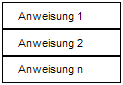
\includegraphics[scale=1]{images/sequenz}\end{center}
	\caption{Die Sequenz im Struktogramm}
	\label{sequenz}
\end{figure}

\begin{figure}
	\begin{center}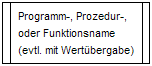
\includegraphics[scale=1]{images/call}\end{center}
	\caption{Der Funktionsaufruf im Struktogramm}
	\label{call}
\end{figure}

\begin{figure}
	\begin{center}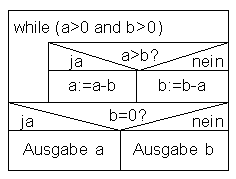
\includegraphics[scale=0.75]{images/example}\end{center}
	\caption{Ein Beispielalgorithmus in Pseudocode}
	\label{example}
\end{figure}

\section{Aufgaben}

\begin{itemize}
	\item Finde heraus welches Problem der gegebene Pseudocode löst.
	\item Schreibe einen Pseudocode, welcher die Weckzeit deines Weckers bestimmt.
	\item Schreibe ein Programm im Pseudocode, lass dir von jemand anderem aus deinem Kurs erklären, was der Code tut.
\end{itemize}
